% \graphicspath{{\subfix{./../../figures/}}}

\begin{figure}[htbp]
    \centering
    \begin{subfigure}[c]{0.9\textwidth}
        \centering
        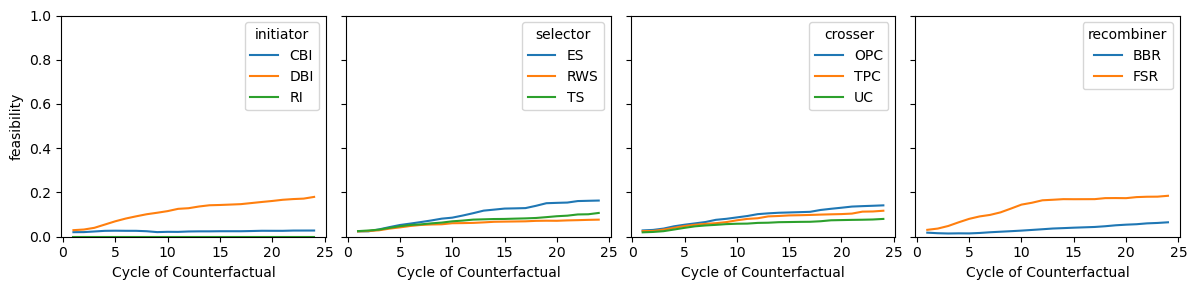
\includegraphics[width=\textwidth]{figures/generated/exp1_feasibility.png}
        \label{fig:exp1-feasibility}    
    \end{subfigure}
    \hfill
    \begin{subfigure}[c]{0.9\textwidth}
        \centering
        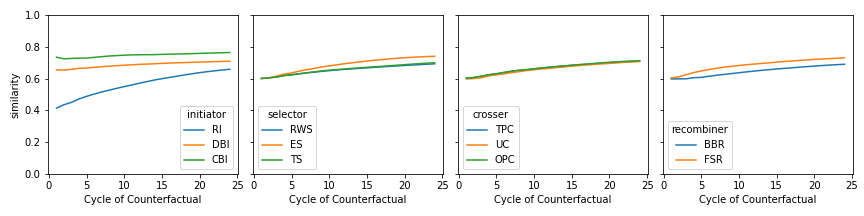
\includegraphics[width=\textwidth]{figures/generated/exp1_similarity.png}
        \label{fig:exp1-similarity}
    \end{subfigure}
    \hfill
    \begin{subfigure}[c]{0.9\textwidth}
        \centering
        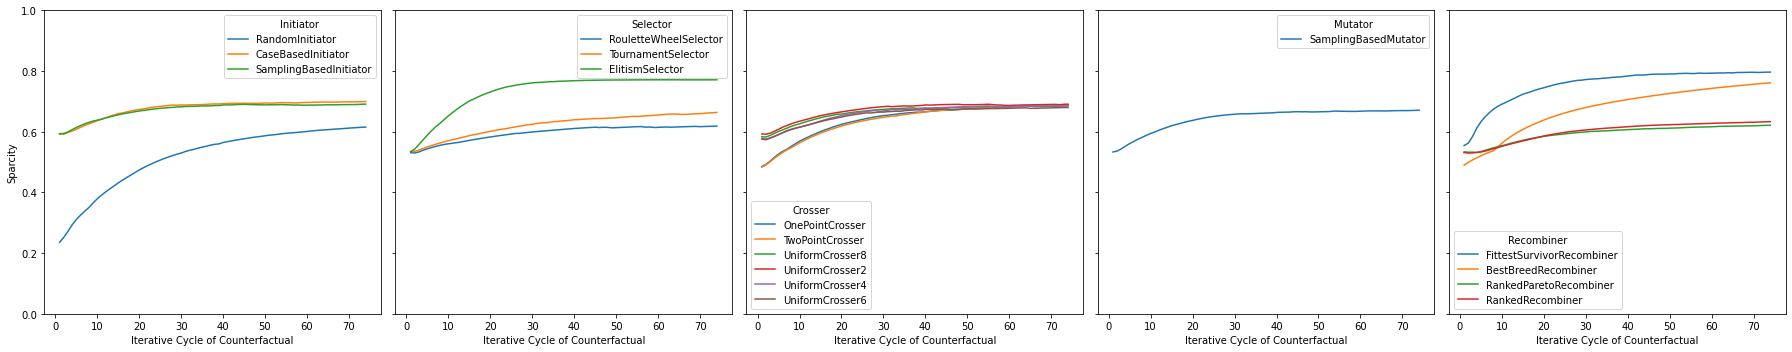
\includegraphics[width=\textwidth]{figures/generated/exp1_sparcity.png}
        \label{fig:exp1-sparcity}
    \end{subfigure}
    \hfill
    \begin{subfigure}[c]{0.9\textwidth}
        \centering
        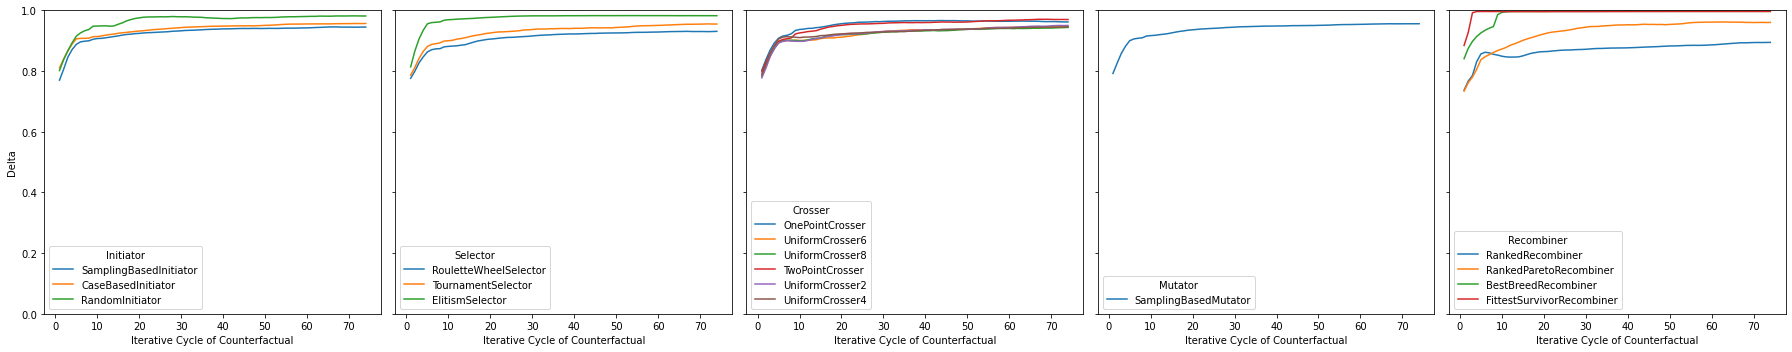
\includegraphics[width=\textwidth]{figures/generated/exp1_delta.png}
        \label{fig:exp1-delta}
    \end{subfigure}
    \caption{Shows the evolution of each viability measure over the entire span of iterative cycles. Each figure adjust the respective operator type by taking the average over all other operator types. \attention{Make sure, that the legends are aligned in color.}}
    \label{fig:exp1-measure}
\end{figure}